\documentclass{llncs} 
\usepackage{url} 
\usepackage{times}
%For math symbols like number classes
\usepackage{amsfonts}
\usepackage{amssymb}
\usepackage{amsmath}
%\usepackage{amsthm}
\usepackage{floatflt}
\usepackage{wrapfig}
\usepackage{multirow}

\usepackage{graphicx}
\usepackage{graphics}

\usepackage[boxed,linesnumbered,vlined,slide]{algorithm2eCustom}

%\usepackage[numbers,sort&compress]{natbib}

\usepackage{color}

\newcommand{\ffh}[1]{\textbf{TODO: \textit{#1}}} 
\newcommand{\baseline}{Baseline \xspace} 
\newcommand{\dynamgrid}{Dynamic Grid \xspace}
\newcommand{\md}{\mdns \xspace}
\newcommand{\mdns}{MD}
\newcommand{\mds}{\mdsns \xspace}
\newcommand{\mdsns}{MDs}
\newcommand{\ls}{\lsns \xspace}
\newcommand{\lsns}{LS}
\newcommand{\lss}{\lssns \xspace}
\newcommand{\lssns}{LSs}
\newcommand{\ff}{\ffns \xspace}
\newcommand{\ffns}{\textsc{FriendLocator}}
\newcommand{\ffs}{\ffsns \xspace}
\newcommand{\ffsns}{\textsc{FriendLocators}}
\newcommand{\hc}{\hcns \xspace}
\newcommand{\hcns}{\texttt{Hide\&Crypt}}
\newcommand{\vl}{\vlns \xspace}
\newcommand{\vlns}{\textsc{VicinityLocator}}
\newcommand{\vls}{\vlsns \xspace}
\newcommand{\vlsns}{\textsc{VicinityLocators}}
\newcommand{\lmg}{\lmgns \xspace}
\newcommand{\lmgns}{LMG}
\newcommand{\lmgs}{\lmgsns \xspace}
\newcommand{\lmgsns}{LMGs}
\newcommand{\ttslong}{\ttslongns \xspace}
\newcommand{\ttslongns}{Trusted Third-party Server}
\newcommand{\tts}{\ttsns \xspace}
\newcommand{\ttsns}{TTS}
\newcommand{\iuns}{IU}
\newcommand{\rfns}{RF}
\newcommand{\iu}{\iuns \xspace}
\newcommand{\rf}{\rfns \xspace}
\newcommand{\iusns}{IUs}
\newcommand{\rfsns}{RFs}
\newcommand{\ius}{\iusns \xspace}
\newcommand{\rfs}{\rfsns \xspace}


\newcommand{\lpar}{(}
\newcommand{\rpar}{)}

\SetKwBlockLRS{LRSBegin}
\newcommand{\funcc}[3]{\emph{\textbf{#1}}\ensuremath{\lpar #2 \rpar} \LRSBegin{#3}}
%\newcommand{\func}[2]{\emph{\textbf{#1}}\ensuremath{\lpar #2 \rpar} \\}


%To change extension of algorithm2e use \algoext{A}, \algoext{B}, \Algoext{}
\newcommand{\algoext}[1]{\renewcommand{\thealgoext}{#1}}
 
 

 
 
%25000	2685185
%50000	4925925
%75000	7129629
%100000	9574074

%------------------------------------------------------------------------- 
% take the % away on next line to produce the final camera-ready version 
\pagestyle{plain}
%
%------------------------------------------------------------------------- 
\begin{document}

\newtheorem{thm}{Theorem}[section]
\newtheorem{cor}[thm]{Corollary}
\newtheorem{lem}[thm]{Lemma}

\SetKwBlockLRS{LRSBegin}


\title{A Location Privacy Aware Friend Locator}
\toctitle{A Location Privacy Aware Friend Locator}
\titlerunning{A Location Privacy Aware Friend Locator}

\author{Laurynas \v{S}ik\v{s}nys
\and Jeppe R. Thomsen
}
\institute{Aalborg University\\ Department of Computer Science \\ Selma Lagerl\o fs Vej 300, DK-9220 Aalborg \O \\ Denmark}
\maketitle

\begin{abstract}
 % All the papers either solve the problem of a more efficient cache in a specific domain, or use the network domain,  which are both relevant, but not really useful when looking at shortest path caching.
% 
% The papers show some interesting ways to use cache, but ultimately their approaches are very domain or query specific so their approaches to caching and cache replacement/invalidation can not be applied directly.


short description of what we do, why this is an interesting/challenging problem, and how well we solve the problem (key results, mention theoretical guaranties.)
\end{abstract}
\section{Introduction} \label{sec:intro}

\subsection{idea for running example}
A user issues two queries as seen in fig. \ref{fig:advancedroutequery}. We can then argue, using this figures and the map in fig. \ref{fig:map10} about all the optimizations we plan to use. (same queries in all figures, and they correspond to map)




\section{Motivation}
Previous work on caching focus on domains which usually has two key characteristics: data locality and limited set of possible items which can be cached (\cite{ref.}). 
There has not been any previous work done developing a caching scheme usable in domains with large set of possible cacheable items and little or no locality in new items added to system, or suggested added to cache. \spath caching is one such domain.. 

\spath calculation is much slower than retrieval from cache, as a cache can supply a \spath directly. 
%where a \spath algorithm will on at most have to visit $AF^{AVN}$ nodes (see table of notation). 
\spath service providers want to spend less money on hardware (\cite{ref.}) and users want fast response time which (\cite{ref.}), when compared to investing in more hardware and bandwith, can be archived in a much cheaper and scalable way by implementing a \spath cache.

Returning a precomputed \spath result is faster, however, it is not feasible to store all possible \spaths. The cache replacement policy of a \spath cache ensures that most queries can be answered by the cache, ensuring as many queries as possible is answered with the space available to the \spath cache.

More users now have a GPS and Web enabled mobile devices which makes \spath services more popular, but also require them to serve much larger set of users.








% 
% \subsubsection{OSC - Optimal Substructure Cache}
% OSC is more advanced than the two previous proposed solutions and therefor the scenario has been updated in figure . 
% To further improve upon Improved Baseline we will again utilize the optimal substructure, making it possible to have much fewer items in cache and still retain a high cache hit percentage \cite{ref}. %(assumption, need test result or proof), 
% Results with sub-paths shared by many users and longer, rather than short, paths are preferred to increase the utility of the cached shortest-path results.
% 
% By adding a more intuitive cache replacement policy which takes in to consideration both the usage of each cache item, as well as the coverage of previously often seen queries it is likely that the utility of the cache would be much higher. This addition is shown with the addition of the "`add to cache"' box in figure \ref{fig:advancedroutequery}B, added to show a heuristic\footnote{the actual heuristic will of cause only be defined later} will be used instead of a very simple method like LRU.


%\paragraph{\textbf{Number 3, ideas}}
%use optimal substructure\\
%prefer having longer paths in cache\\
%prefer having paths with subpaths shared by many users\\
%look at utility of cache items, not just usage when designing cache replacement policy.\\
%\begin{itemize}
%\item	prefer often used cache items
%\item	prefer items which cover routes/areas often used in previous queries
%\end{itemize}





%\paragraph{crap}
%We assume a setting where all users are equipped
%with a Mobile Device (MD) able to communicate and
%report the users position. All MDs are online and are
%continuesly reporting the users location at predetermined
%intervals. We use the terms user, mobile device, and
%client interchangeable and denote the set of MDs by
%UN. We expect a MD to be cabable of visualizing
%its current location.
%We assume a 2D scenario, where the movements of
%users uU are restricted to a road network G(V, E).
%V is the set of vertices, where each vertice v ∈ V
%represents either a street intersection or an important
%landmark. E is the set of directed edges augmented
%by edge length and type. Edges are represented by
%a begin/end vertice pair and each edge represents the
%smallest unit of a road segment. e ∈ E, each e being
%a tuple specifying id, start-/end-vertices, length, and
%Road Type (RT) (eid , vs , ve , elength , eRT ). RT is a
%hierarchy of the size/type of road i.e. highway, paved,
%or dirt road (Sec. 5.2).
%The simplest form of trajectory is a collection of tu-
%ples (time, longitude, latitude), ordered by the time
%attribute, but as we will work on a road network and
%in the spatio-temporal domain, such a basic notion of
%trajectories is not appropriate. We define T as the set
%of trajectories, where each trajectory consist of an id
%(tid ), and a sequence of tuples containing an edge and




\section{Related Work} \label{sec:rel_work}
%
In this section we review general location privacy preserving techniques 
followed by the relevant work on location privacy in proximity detection
services.

\subsection{General Location Privacy Techniques}

In the most common setting assumed in location-privacy research,
an LBS server maintains a public set of points-of-interest (POI), e.g. gas
stations. The goal is then to retrieve from the server the nearest POIs to the
user, without revealing the user's location $q$ to the server. Many
location privacy solutions exist for this setting and they can be broadly
classified into two categories: spatial cloaking and transformation. 

Spatial cloaking \cite{gruteser03,mca06,duckham05a,acdvs07} techniques
generalize the user's exact location $q$ into a region $Q'$, which is then used
for querying the server. The region $Q'$ is then sent to the LBS server, which
returns all the results that are relevant to any point in $Q'$. Such technique
ensures that even if the attacker knows locations of all users, the identity of
the querying user can be inferred only with some probability. 

The transformation approaches \cite{ks07,ghinita08} map the user's location $q$
and all POIs to a transformed space, in which the LBS server evaluates queries
blindly without knowing how to decode the corresponding real locations of the
users.

In contrast, in the proximity detection problem, the users' locations are both
query locations and points-of-interest that must be kept secret. Thus the
existing spatial cloaking and transformation techniques, that assume public
datasets, cannot be directly applied for proximity detection. However the
concepts of spatial cloaking and transformation can be, and are used in the
existing privacy-aware proximity detection approaches.

\subsection{Privacy-aware proximity detection methods}

Ruppel et al. \cite{proxDetTrans} develop a centralized solution that supports
proximity detection with a certain level of privacy. It applies a distance-preserving 
mapping (a rotation followed by a translation) to convert the user's location $q$ into 
a transformed location $q'$. Then, a centralized proximity detection method is 
applied to detect the proximity among those transformed locations. However, Liu 
et al. \cite{lgk06} points out that such distance-preserving mapping is not safe 
and a attacker can easily derive the mapping function and compute the users' original 
locations. 

% maybe remove???
Mascetti et al. present a centralized solution
\texttt{Longitude} \cite{longitudePaper}.
Here users apply spatial cloaking followed by modular transformation prior
sending their 
locations the server. The applied transformation prevents the disclosure of 
location information, but introduces false proximity detections that do not occur in our 
proposed approach.


\hc, presented in \cite{pbsPaper}, is a privacy preserving solution which employ
the filter-and-refine paradigm. First, users spatially cloak their locations and sent them the
server. Then, the server computes a minimum and maximum distances (Fig. \ref{fig:relworkDemos}a)
between these cloaking regions. Depending on the specified thresholds and computed distances, 
the server classifies friends being in, not-in, or possibly-in proximity. The classification 
result is immediately reported to users, and in case of uncertainty, two users have to perform 
direct communication in order to refine their proximity status. 
In the refinement step first two users map their locations 
and vicinity regions into the some spatial subdivision, e.g. grid, and then they use secure 
two-party computation protocol to check if the mapped location of one user lays inside the 
mapped vicinity of other user. This can be performed with no need for the users 
to expose their mapped locations and vicinities. Depending on the result of the 
set-inclusion checking, either proximity or separation is detected. Figure
\ref{fig:relworkDemos}b visualizes a scenario, where user $u_2$'s grid-mapped location
(dark rectangle) intersect with $u_1$'s grid-mapped vicinity region. In this case, 
the proximity between $u_1$ and $u_2$ is detected.

Unlike in our approach, their proposal does not completely hide user locations
from the central server as it always knows their cloaked regions. If strong
privacy is required users are forced to perform user-to-user communication more
frequently thus significantly increasing the amount of client communication due to
an expensive secure two-party computation protocol. 



\begin{figure}
       \center
       \begin{tabular}{cc}
			   
\includegraphics[width=0.25\textwidth]{vl/images/pbsDemo.pdf} &
			   
\includegraphics[width=0.18\textwidth]{vl/images/pbsDemo2.pdf} \\
%	Filtering step & Refinement step \\
          (a) & (b) \\
\includegraphics[width=0.15\textwidth]{vl/images/proxDetDemo.pdf} &
{\scriptsize %\footnotesize
     \begin{tabular}[b]{| c | c |}\hline
        \textbf{Col/ Row} & \textbf{$\mathbf{\Psi}$} \\  \hline
        0 & $c_0$ (5)\\ \hline
        1 & $c_1$ (9)\\ \hline
        2 & $c_2$ (1)\\ \hline
        3 & $c_3$ (7)\\ \hline	
     \end{tabular}
} \\
          (c) & (d)
       \end{tabular}
       \caption{Behavior of \hc and \ff}
            \label{fig:relworkDemos}
\end{figure}



\v{S}ik\v{s}nys et al. \cite{ffinder} have developed a centralized privacy-aware
proximity detection method, called \ff, which provides strong privacy guaranties
and employs a grid-based technique to optimize communication cost. 
Users map their locations into 4 cells of the grid from a \textit{list of grids},
and, prior sending to the server, encrypt them using shared, one-to-one mapping encryption function.
The \textit{list of grids} globally defines a collection of grids, where cell sizes of distinct grids 
monotonically decreases with respect to the \textit{level number}. The server is able to 
perform a matching between encrypted coordinates of different users, for a shared
level, and report the matching result. When matchings at all consecutive levels 1
to $L_{max}$ are detected then actual proximity between two users is detected.
Pairs of users individually choose $L_{max}$ value which yields a
specific mutual vicinity radius for two users. The proximity is detected
iteratively such that after each encrypted coordinate match, 
the server checks if required level $L_{max}$ is reached. If so, then users are
informed about their proximity, otherwise the server sends a message to one or
both of the users asking them to use a finer grid, i.e., increase their current
level, for the next matching iteration. 

E.g. if the encryption function $\Psi$ is as defined in
\ref{fig:relworkDemos}d, then encrypted coordinates of users $u_1$, $u_2$, and
$u_3$ respectively are $(x:[c1,c2],y:[c0,c1])$, $(x:[c2,c3],y:[c1,c2])$,
$(x:[c0,c1],y:[c2,c3])$. Assuming that level of grid in Fig.
\ref{fig:relworkDemos}c is $L_{max}$, the user $u_1$ is in proximity with $u_2$,
however $u_3$ is not in proximity with either.



The limitation of the \ff is low, and uncontrollable, precision of the
proximity detection. On the proximity notification the actual distance between
two users can be any in the range from $d$ to $d + \lambda$, 
where $d$ is width/height of grid cell at level $L_{max}$, 
$\lambda = d(2\sqrt(2) - 1)$ is a service precision parameter. Note, 
that in most other proximity detection approaches, unlike in \ff, the parameter 
$\lambda$ can be chosen freely by users. 

None of the existing privacy-aware approaches directly support the ``river'' 
and the ``bar'' proximity detection scenarios (see Fig. 
\ref{fig:suppVic}c/\ref{fig:suppVic}d) since they use static circular-shape vicinity. 
However some solutions, like \hc \cite{pbsPaper}, might be adapted to support dynamic 
vicinities, though current limitations will persist and introduce new problems 
like e.g. how to efficiently update user locations and vicinities.




\subsection{Our contribution}

In this work we combine best features of the previously presented proximity
detection approaches to build our solution, the \vl. The solution combines the
ideas of encrypted coordinates, their blind matching at the server-side, and
the vicinity mapping into multi-spatial subdivisions, e.g. list of grids.
Our solution, unlike Mascetti et al. \cite{pbsPaper} proposal, employs only
centralized architecture, where the server knows no users' spatial data. It
allows users individually select preferable proximity detection precision and 
supports irregular-shape, changing over time vicinities. Our proposal
is will be targeted for 2D environment.
It can however easily be generalized to n-dimension.

\section{Problem}\label{sec:problem}

In our setting we assume users own an Internet enabled mobile device with positioning capabilities. Users issue \spath queries to an online service provider. Users want the response time, on the return of their \spath result, to be comparable to that of an offline application. We use the terms user query, incoming query, and query interchangeably.

The \spath service provider needs to provide a fast service to its users. The service provider also want to save cost on hardware, such as CPU and HDD space. The \spath provider therefor wants to return as many \spath results as possible, using the least amount of computation and space.

Calculating a \spath will, regardless of the algorithm used, always be an expensive calculation\cite{CNeed}. Using a \spath cache at the \spath service provider can reduce the CPU cycles used in order to return a \spath result. Doing so would at the same time also increase the response time of the \spath service, as saving CPU cycles not only allows for more \spaths to be computed on the same hardware, but also allows for returning a cached result much faster than it would be possible if the \spath had to be calculated first.

A \spath has the property of \oss (see lemma \ref{lem:oss}) which means that any \spath in the cache can answer any \spath query where both origin and target node are on the \spathns. Calculating which \spathsns, and their sub-paths, provide the most benefit will obviously be necessary for optimal utilization of the cache. A static cache, which is populated in an offline phase (fig. \ref{fig:routequery}E), is used. A static cache will impose minimal overhead to query processing. Section \ref{sec:competitors} explains why we choose a static cache.

The properties of \ossns (Lemma \ref{lem:oss}) states that all sub-paths on a \spath are also \spathsns. Using \spath Q1 in table \ref{tab:queries} we would also be able to a query from $v_3$ to $v_5$, or $v_4$ to $v_6$ (See fig. \ref{fig:rxmap}), as these nodes are part of Q1. The same of cause also holds for any \spath Q1-Q6 from table \ref{tab:queries}.

\begin{figure}[hbt]
  \center
        \includegraphics[width=0.5\textwidth]{figures/rxmap}
        \caption{Simple graph representation of a map.}
  \label{fig:rxmap}
\end{figure}


\subsection{Architecture}
We propose a system with a static \spath cache implemented in front of an existing \spath service (See fig. \ref{fig:routequery}) such that if the cache can answer a query then the result can be returned immediately. 

When the system receives a \spath query from a user (fig. \ref{fig:routequery}A) the system first checks if the cache (fig. \ref{fig:routequery}B) is able to answer the query. If the cache contains the query answer it is immediately returned (fig. \ref{fig:routequery}D), else the \spath algorithm is called (fig. \ref{fig:routequery}C) and the \spath result returned (fig. \ref{fig:routequery}D).

\begin{figure}
  \center
        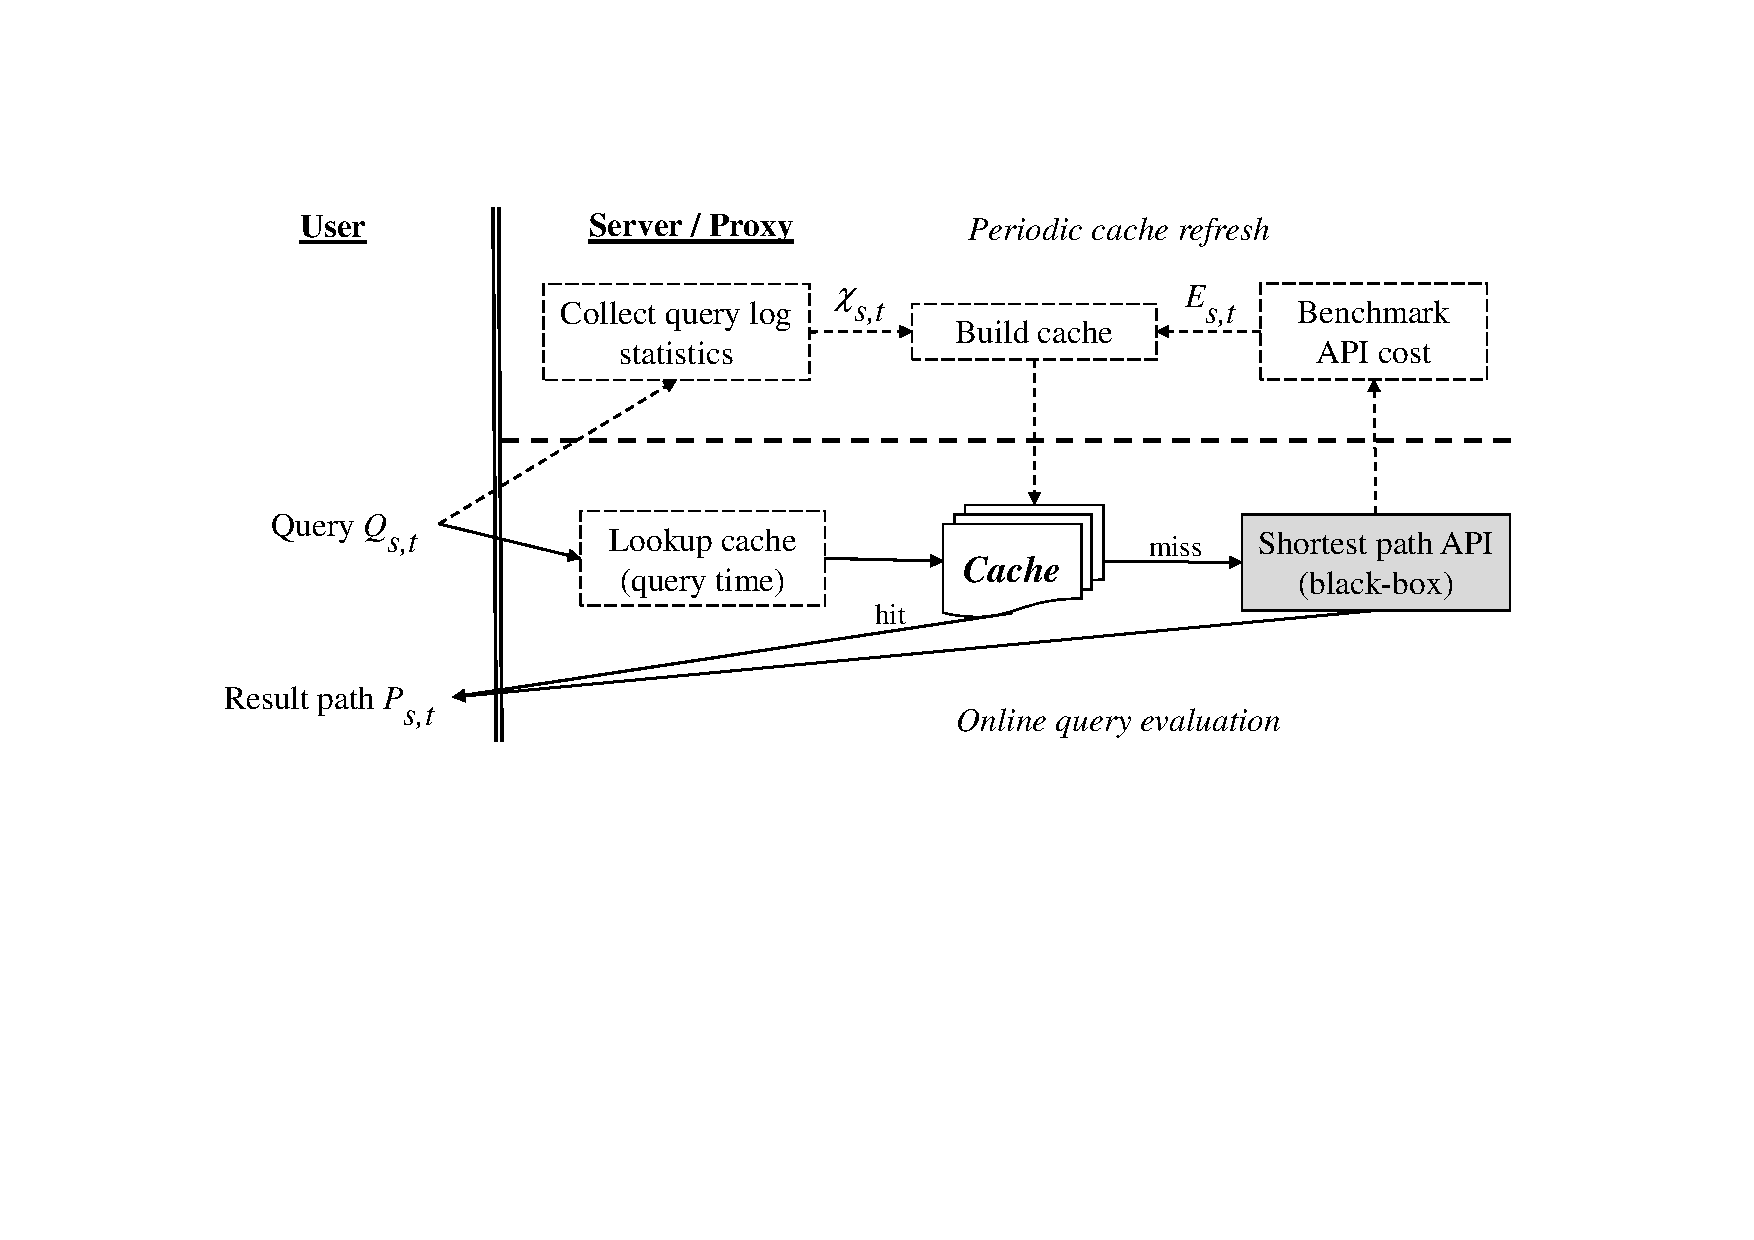
\includegraphics[width=0.5\textwidth]{figures/routequery}
        \caption{Buffer placement in \spath service providers system.}
  \label{fig:routequery}
\end{figure}


\subsection{Optimization Intend} \label{subsec:goals}

As the main problem with expensive \spath calculations is time needed, we use reduction in \textit{\cet} as the main optimization target and measurement to evaluate our success.
At a \spath service provider, the time spent to return a \spath result is essentially composed of two tasks: calculating the \spath and the overhead of query processing. 

We will address 3 subgoals:
\begin{enumerate}
\item \label{item:goal1}Reduce the gross \cet used to calculate \spathsns.
\item \label{item:goal2}Reduce the gross \cet spent on overhead in query processing.
\item \label{item:goal3}Determine the value of a sub-path in the cache.
\end{enumerate}

We want reduce the gross \cet of \spath calculations - goal 1 - as it is the most CPU intensive task at a \spath service, and therefor also the most time consuming. By using a cache we expect to see a negavite correlation between cache hit rate and \cet used on \spath calculation.

In a \spath service there will always be a some overhead associated with \spath query processing. Introducing a cache in front of the existing \spath service (fig. \ref{fig:routequery}B) will undeniably add more overhead as the cache needs to be queried for all queries submitted to the \spath service, regardless of whether it is able to answer the query or not. In order for the cache to be useful, the overhead introduced needs to be minimized (goal \ref{item:goal2}). We always have to make sure that the savings achieved by adding a cache to the system is greater than the overhead introduced.

The fact that the system will be using a static cache, and \spaths exhibit the \oss property, makes goal 3 - determining the value of a \spath subpath - very important. The ability to do goal \ref{item:goal3} well will have a direct influence on goal \ref{item:goal1} and  \ref{item:goal2}. If we fill the cache with useless \spaths we will end up calculating a \spath for all queries, as well as the overhead from checking the cache for each query. Solving goal 3 well is the most direct way to solve goal 1.

The \oss property states that every sub-path of a \spath is also a \spath. i.e \spath Q1 in table \ref{tab:queries} consists of: 
$\{Q_{1,3}, Q_{1,4}, Q_{1,5}, Q_{1,6}, Q_{3,4},$ $Q_{3,5}, Q_{3,6}, Q_{4,5}, Q_{4,6}, Q_{5,6}\}$, each one being a \spathns.

\begin{lemma}\label{lem:oss}
If a path $Q_{s,t}: v_s,v_{s+1},\ldots,v_t$ is a \spath, then $\forall$ $(v_k,v_l) | v_k \in Q_{s,t} \wedge v_l \in Q_{s,t}$ there is a  \spath $Q_{k,l}$ with start-/end-node in $v_k,v_l$, following a sub-path of $Q_{s,t}$ 
\end{lemma}

\begin{table}
\begin{tabular*}{\columnwidth}{|l||p{0.69\columnwidth}|}
\hline
\bf Abbreviation & \bf Meaning \\\hline
\spath          & Shortest Path \\\hline
$Q_{s,t}$	& \spathns: $\{v_s,v_{s+1},\ldots,v_t\}$ \\\hline
\acs{LRU}       & \acl{LRU} \\\hline
FIFO            & First In First Out \\\hline
\acs{SPS}       & \acl{SPS} \\\hline
\acs{CET}	& \acl{CET} \\\hline
\acs{OSS}	& \acl{OSS} \\\hline
\end{tabular*}
\caption{Table of Notation}
\label{tab:symbols}
\end{table}




% \subsection{helping text}
% \begin{enumerate}
% \item Introduce the problem setting in more detail than in the introduction and formally define the problem and what exactly we aim to solve in this paper.\\
% \item show where exactly the proposed cache is located in an online \spath service providers system.
% \item State goal 1(a) and 2(b)
% 	\begin{enumerate}
% 	\item Reduce the time spent executing the \spath algorithm. - The \spath algorithm is usually the single most CPU expensive task at a \spath service provider.
% 	\item Reduce the time spent on overhead. - Introducing a cache will also add some overhead, this overhead not desirable and should  be minimized.
% 	\end{enumerate}
% \item Introduce the overall setting which our solution work in and give a table of notation for reader reference.
% \end{enumerate}
%
\section{Contribution}

\subsection{Statistics Extraction}

\begin{frame}[shrink=10] %hmm.. thought i could change colour here :S
\frametitle{Statistics Extraction} 


    \begin{tabular}{ccc}
\begin{tabular}{@{}|c@{}|c@{}|@{}}
\hline
Timestamp & Query \\ \hline 
$T_1$ & $Q_{3,6}$ \\ \hline 
$T_2$ & $Q_{1,6}$ \\ \hline 
$T_3$ & $Q_{2,7}$ \\ \hline 
$T_4$ & $Q_{1,4}$ \\ \hline 
$T_5$ & $Q_{4,8}$ \\ \hline 
$T_6$ & $Q_{2,5}$ \\ \hline 
$T_7$ & $Q_{3,6}$ \\ \hline  
$T_8$ & $Q_{3,6}$ \\ \hline 
\end{tabular}
&
    \begin{tabular}{|@{ }c@{ }|@{ }c@{ }c@{ }c@{ }c@{ }c@{ }c@{ }c@{ }c@{ }|}
       \hline
       $\chi_{s,t}$	& $v_1$	& $v_2$	& $v_3$	& $v_4$	& $v_5$	& $v_6$	& $v_7$ & $v_8$ \\\hline
       $v_1$			& /	& 0	& 0	& 1	& 0	& 1	& 0	& 0	 \\
       $v_2$			& 0	& /	& 0	& 0	& 1	& 0	& 1	& 0	 \\
       $v_3$			& 0	& 0	& /	& 0	& 0	& 3	& 0	& 0	 \\
       $v_4$			& 1	& 0	& 0	& /	& 0	& 0	& 0	& 1	 \\
       $v_5$			& 0	& 1	& 0	& 0	& /	& 0	& 0	& 0	 \\
       $v_6$			& 1	& 0	& 3	& 0	& 0	& /	& 0	& 0	 \\
       $v_7$			& 0	& 1	& 0	& 0	& 0	& 0	& / & 0  \\
       $v_8$			& 0	& 0	& 0	& 1	& 0	& 0	& 0 & /  \\
       \hline
    \end{tabular}
	\\
    \end{tabular}\\

\hspace{10em}\includegraphics[width=0.55\columnwidth]{images/rxmap} 


\end{frame}

\begin{frame}[shrink=10] %hmm.. thought i could change colour here :S
\frametitle{Grouping} 

\begin{tabular}{lc}

    \begin{tabular}{|@{ }c@{ }|@{ }c@{ }c@{ }c@{ }c@{ }c@{ }c@{ }c@{ }c@{ }|}
       \hline
       $\chi_{s,t}$	& $v_1$	& $v_2$	& $v_3$	& $v_4$	& $v_5$	& $v_6$	& $v_7$ & $v_8$ \\\hline
       $v_1$			& /	& 0	& 0	& 1	& 0	& 1	& 0	& 0	 \\
       $v_2$			& 0	& /	& 0	& 0	& 1	& 0	& 1	& 0	 \\
       $v_3$			& 0	& 0	& /	& 0	& 0	& 3	& 0	& 0	 \\
       $v_4$			& 1	& 0	& 0	& /	& 0	& 0	& 0	& 1	 \\
       $v_5$			& 0	& 1	& 0	& 0	& /	& 0	& 0	& 0	 \\
       $v_6$			& 1	& 0	& 3	& 0	& 0	& /	& 0	& 0	 \\
       $v_7$			& 0	& 1	& 0	& 0	& 0	& 0	& / & 0  \\
       $v_8$			& 0	& 0	& 0	& 1	& 0	& 0	& 0 & /  \\
       \hline
    \end{tabular}
&
\multirow{3}{*}{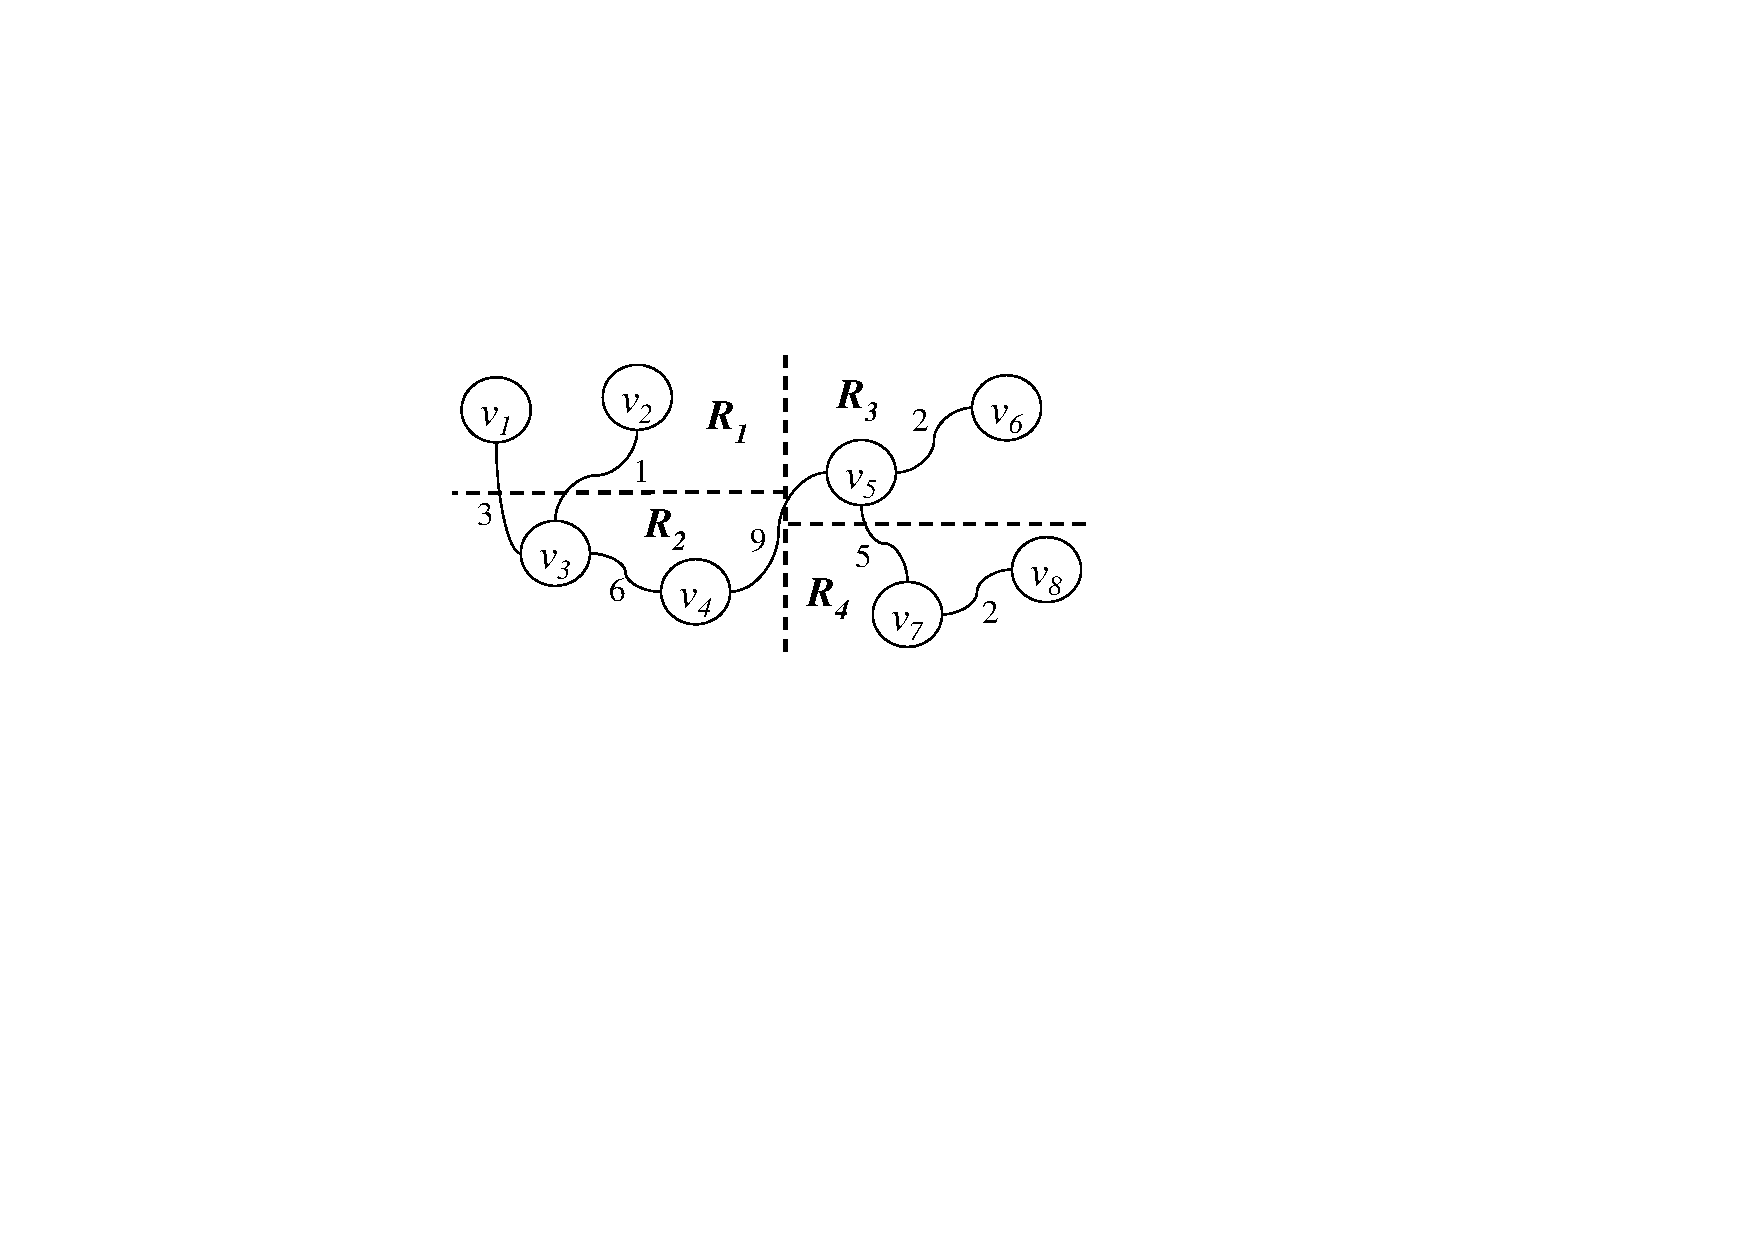
\includegraphics[width=0.68\columnwidth]{images/mappartition}} \\
& \\

	\begin{tabular}{|@{ }c@{ }|@{ }c@{ }c@{ }c@{ }c@{ }|}
	\hline \small
	\textbf{$\chi_{R_i,R_j}$}	& $R_1$		& $R_2$		& $R_3$		& $R_4$\\\hline
	$R_1$			& 0	& 1	& 2	& 1 \\ 
	$R_2$			& 1	& 0	& 3	& 1 \\ 
	$R_3$			& 2	& 3	& 0	& 0 \\ 
	$R_4$			& 1	& 1	& 0	& 0 \\ 
	\hline
	\end{tabular}
	\\
&
% \multicolumn{2}{c}{\includegraphics[width=0.75\columnwidth]{images/rxmap}}
  
\end{tabular}

\end{frame}




\subsection{Cost Estimation}
\begin{frame}[red] %hmm.. thought i could change colour here :S
\frametitle{SP Call Cost Estimation} 


\begin{columns}[b]
  \begin{column}{0.5\textwidth}
\begin{exampleblock}{Proxy Scenario}
$E_{s,t}(Proxy) = 1$
\end{exampleblock}

\begin{exampleblock}{Server Scenario}
Intuition: Longer query results incur higher cost.
\end{exampleblock}

$-$ Cost only estimated in server scenario\\
$-$ Estimation methods developed for Server scenario
  \end{column}
  \begin{column}{0.45\textwidth}

  \end{column}
\end{columns}


  \begin{picture}(0.0,0.0) 
     \put(160,30){  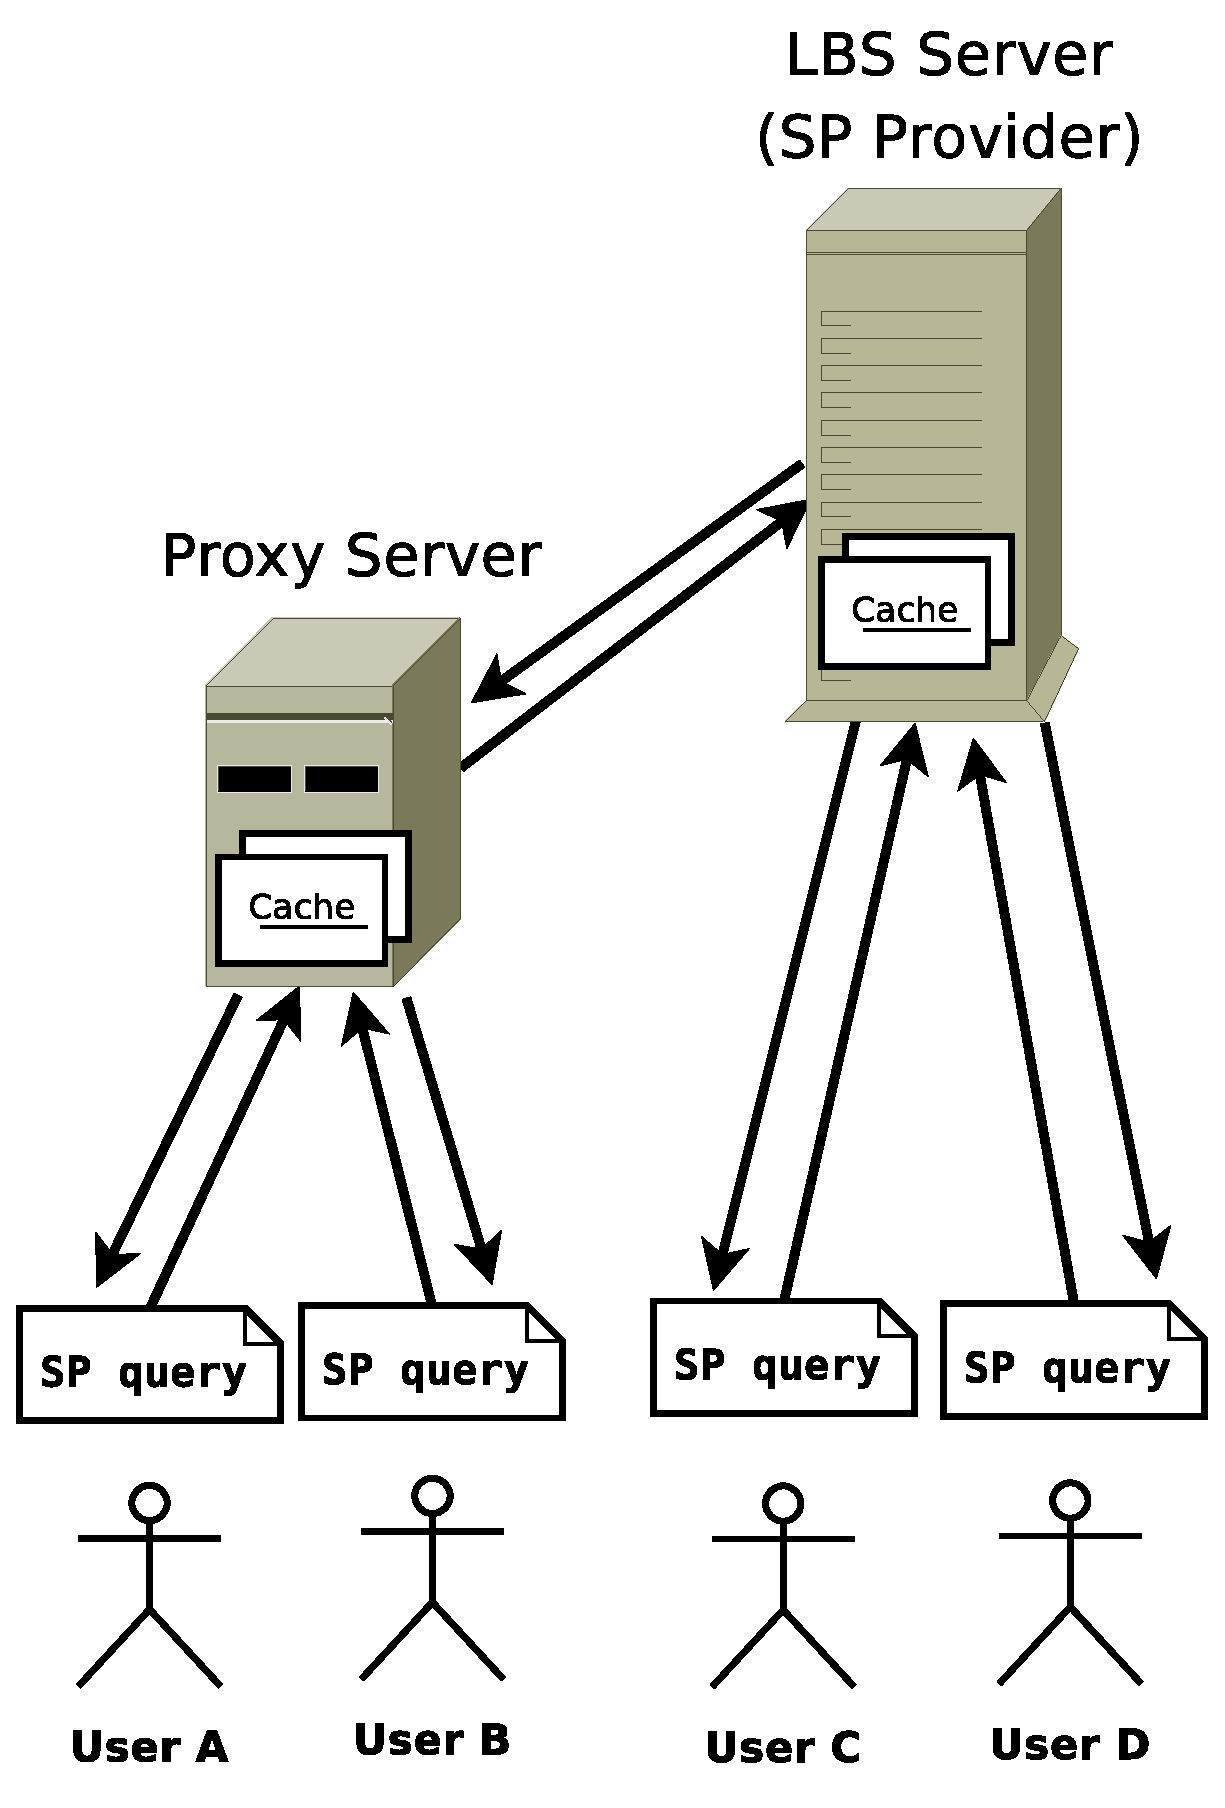
\includegraphics[width=0.5\textwidth]{images/scenario} }
  \end{picture}



% Two data structures:
% \begin{itemize}
%   \item Distance estimator, Landmark-based [Potamias et al. CIKM]
%   \item Expense histogram
% \end{itemize}
\end{frame}


\subsection{Benefit Model}



\begin{frame} %hmm.. thought i could change colour here :S
\frametitle{Incremental Benefit per size} 
  \begin{block}{Benefit formula}
    $\Delta\overline{\gamma}(P_{a,b}, \Psi) = \sum\limits_{P_{s,t} \in \mathfrak{U}(P_{a,b}) - \mathfrak{U}(\Psi)} \frac{\chi_{s,t} * E_{s,t}}{|P_{a,b}|}$
  \end{block}


\begin{itemize}
\item $P_{a,b}$: a shortest path 
\item $\Psi$: the cache 
\item $\mathfrak{U}(P_{a,b})$: all sub-paths of $P_{a,b}$. 
\item $\chi_{s,t}$ frequency of query $s$ to $t$. 
\item $E_{s,t}$: cost of calculating $P_{s,t}$
\end{itemize}

\end{frame}

% \begin{frame} %hmm.. thought i could change colour here :S
% % \frametitle{Benefit Model} 
% 
% \begin{columns}
%   \begin{column}{0.4\textwidth}
% From Query Log:
%   \begin{tabular}{|l|l|}
%     Shortest Path & Frequency \\\hline
%     $P_{3,6}$ & 3 \\
%     $P_{1,4}$ & 1 \\
%     $P_{1,6}$ & 1 \\
%   \end{tabular}
%   \end{column}
%   \begin{column}{0.1\textwidth}
%   \end{column}
%   \begin{column}[t]{0.6\textwidth}
% Cost Estimation:\\
%   \begin{tabular}{|l|l|}
%     Shortest Path & Cost \\\hline
%     $P_{3,6}$ & 3 \\
%     $P_{1,4}$ & 2 \\
%     $P_{1,6}$ & 4 \\
%   \end{tabular}
%   \end{column}
% \end{columns}
% 
% 
%     \includegraphics[width=0.4\textwidth]{images/rxmap} 
% 
%     \hspace{-2em}$\gamma(\Psi)=1*2+1*4+3*3=15$\\
% 
%   \begin{exampleblock}{$\gamma(P_{1,6}) + \gamma(P_{3,6}) \neq \gamma(\Psi)$}
% \hspace{0.7em} (15) \hspace{1.8em} (9)
%   \end{exampleblock}
% \end{frame}


\begin{frame}[shrink=5]  %hmm.. thought i could change colour here :S
\frametitle{Cache: SP Result Ranking} 

 Greedy algorithm


{\small
\begin{tabular}{@{}|c@{}|c@{}|@{}}
\hline
Timestamp & Query \\ \hline 
$T_1$ & $Q_{3,6}$ \\ \hline 
$T_2$ & $Q_{1,6}$ \\ \hline 
$T_3$ & $Q_{2,7}$ \\ \hline 
$T_4$ & $Q_{1,4}$ \\ \hline 
$T_5$ & $Q_{4,8}$ \\ \hline 
$T_6$ & $Q_{2,5}$ \\ \hline 
$T_7$ & $Q_{3,6}$ \\ \hline  
$T_8$ & $Q_{3,6}$ \\ \hline 
\end{tabular}
}


  \begin{picture}(0.0,0.0) 
     \put(90,5){  \includegraphics[width=0.7\textwidth]{images/rxmap} }
  \end{picture}



{\small
\begin{tabular}{|c||c|c|c|c|c|c||c|c|}\hline
    Round & \multicolumn{6}{c||}{Path} & \multicolumn{2}{@{ }c@{ }|}{Cache $\Psi$ }  \\ \cline{2-9}
             	& $P_{1,4}$ & $P_{1,6}$ & $P_{2,5}$ & $P_{2,7}$ & $P_{3,6}$ &  $P_{4,8}$ & Before &  After 	 	 \\\hline \hline
    1	&  1/3    & \zebox{\bf 5/5}	 & 1/4    & 2/5 &  3/4    & 1/4 &  empty    & $P_{1,6}$ \\\hline
    2	&      &  &     &  &     &  & $P_{1,6}$    & $P_{1,6}, {\bf ?}$  \\\hline
\end{tabular}
}
\end{frame}


\begin{frame}[shrink=5]  %hmm.. thought i could change colour here :S
\frametitle{Cache: SP Result Ranking - Incremental benefit} 


Incremental benefit calculation



{\small
\begin{tabular}{@{}|c@{}|c@{}|@{}}
\hline
Timestamp & Query \\ \hline 
$T_1$ & $Q_{3,6}$ \\ \hline 
$T_2$ & $Q_{1,6}$ \\ \hline 
$T_3$ & $Q_{2,7}$ \\ \hline 
$T_4$ & $Q_{1,4}$ \\ \hline 
$T_5$ & $Q_{4,8}$ \\ \hline 
$T_6$ & $Q_{2,5}$ \\ \hline 
$T_7$ & $Q_{3,6}$ \\ \hline  
$T_8$ & $Q_{3,6}$ \\ \hline 
\end{tabular}
}


  \begin{picture}(0.0,0.0) 
     \put(90,5){  \includegraphics[width=0.7\textwidth]{images/rxmap} }
  \end{picture}



{\small
\begin{tabular}{|c||c|c|c|c|c|c||c|c|}\hline
    Round & \multicolumn{6}{c||}{Path} & \multicolumn{2}{@{ }c@{ }|}{Cache $\Psi$ }  \\ \cline{2-9}
             	& $P_{1,4}$ & $P_{1,6}$ & $P_{2,5}$ & $P_{2,7}$ & $P_{3,6}$ &  $P_{4,8}$ & Before &  After 	 	 \\\hline \hline
    1	&  1/3    & \zebox{\bf 5/5}	 & 1/4    & 2/5 &  3/4    & 1/4 &  empty    & $P_{1,6}$ \\\hline
    2	&  0    & 0 &  1/4    & \zebox{\bf 2/5} &  0    & 1/4 & $P_{1,6}$    & $P_{1,6}, P_{2,7}$  \\\hline
\end{tabular}
}
\end{frame}


\subsection{Data Structure}
\begin{frame}[red] %hmm.. thought i could change colour here :S
\frametitle{Efficient Data Structure for the Cache} %Maybe a figure to easily explain the main point

\begin{itemize}
\item Lookup time grows with size cache 
\item Support return of full or partial cache items
\item Compact storage of shortest paths
\end{itemize}

\begin{figure}[hbt]
  \center %\small
  \begin{tabular}{@{}c@{}c@{ }c@{}}
    \begin{tabular}{c|l|}
        \cline{2-2}
        $\Psi_1$ & $v_1, v_3, v_4$ \\ \cline{2-2}
        $\Psi_2$ & $v_1, v_3, v_2$ \\ \cline{2-2}
        $\Psi_3$ & $v_2, v_3, v_4, v_5$ \\ \cline{2-2}
%        $\Psi_4$ & $v_3, v_4, v_5, v_6$ \\ \cline{2-2}
%        $\Psi_5$ & $v_3, v_4, v_5, v_7$ \\ \cline{2-2}
    \end{tabular}
    &
    \begin{tabular}{c|l|}
        \cline{2-2}
        $v_1$ & $\Psi_1, \Psi_2$ \\ \cline{2-2}
        $v_2$ & $\Psi_2, \Psi_3$ \\ \cline{2-2}
        $v_3$ & $\Psi_1, \Psi_2, \Psi_3$ \\ \cline{2-2}
        $v_4$ & $\Psi_1, \Psi_3$ \\ \cline{2-2}
        $v_5$ & $\Psi_3$ \\ \cline{2-2}
    \end{tabular}
  &
    \begin{tabular}{c}
    \\
    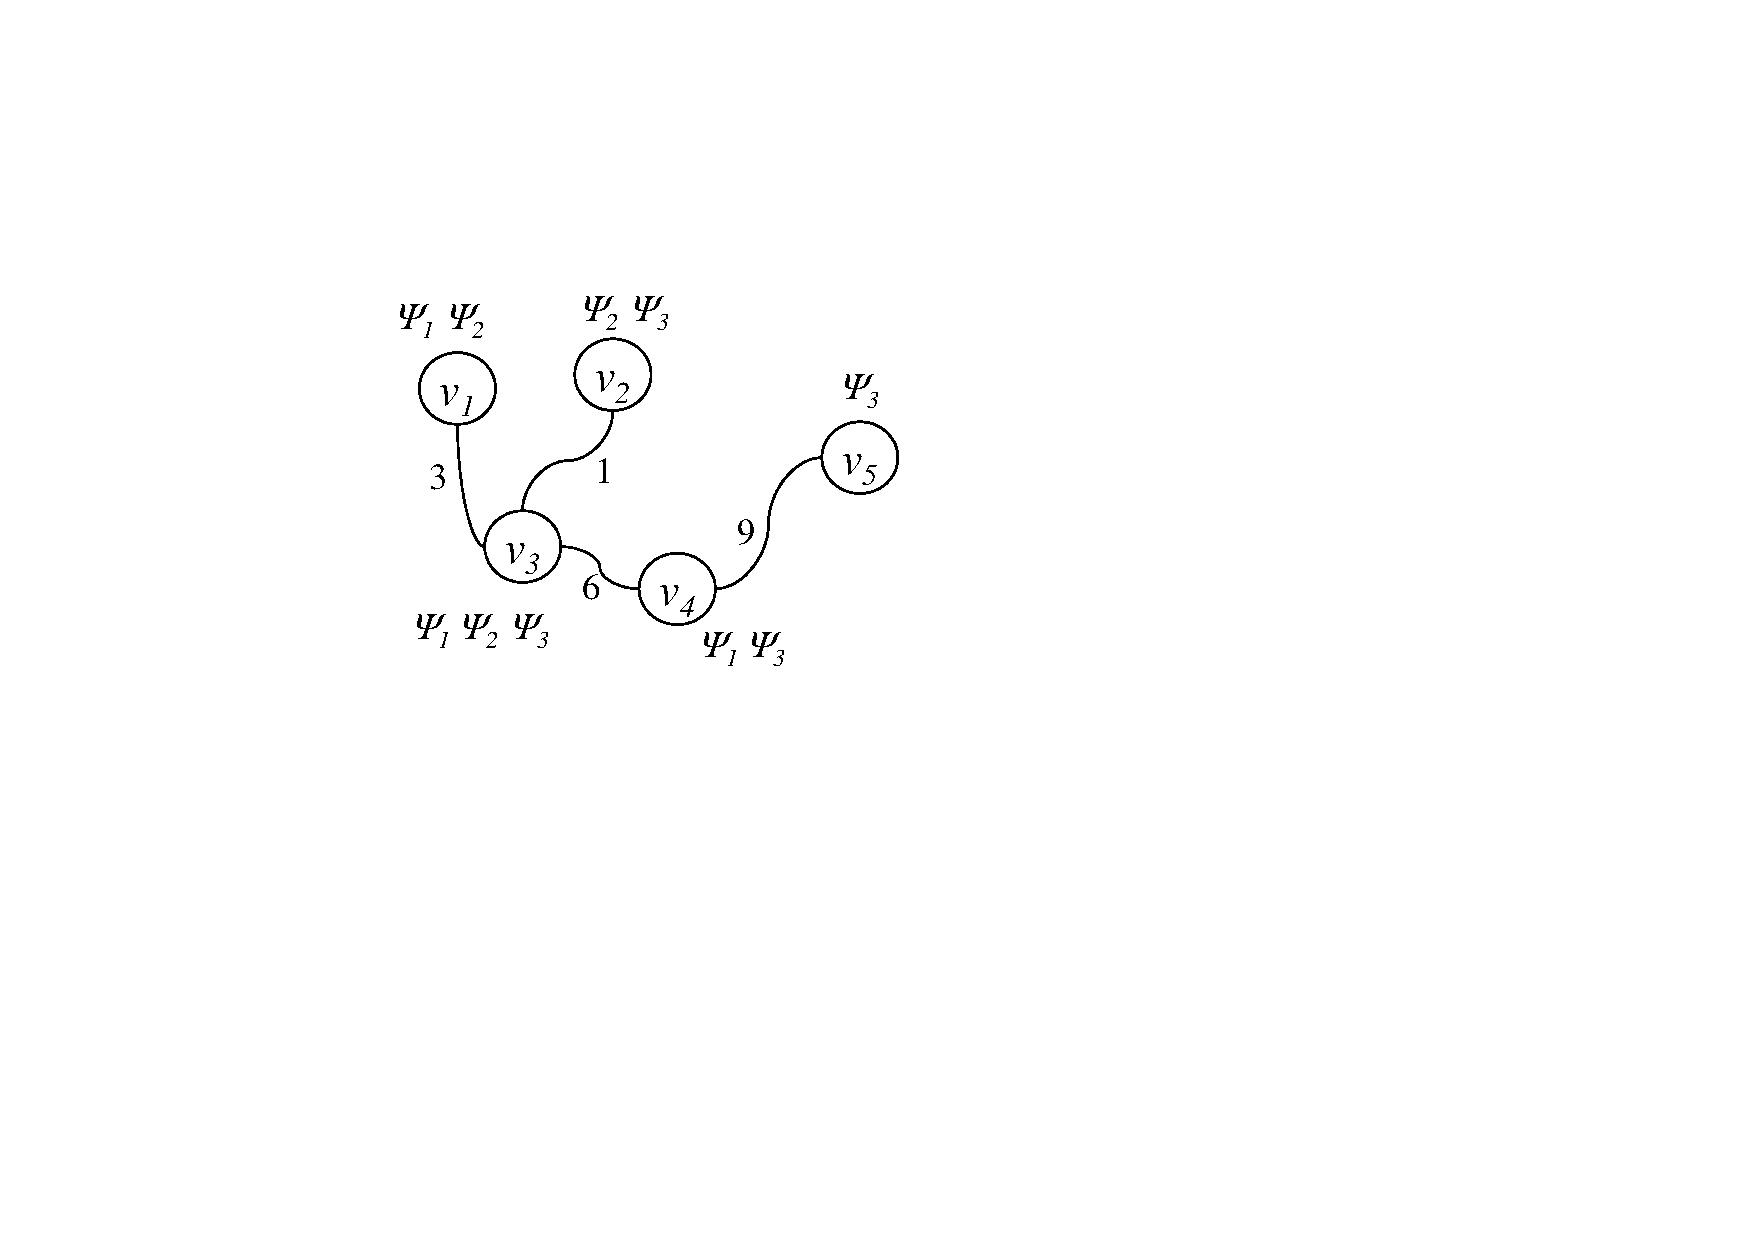
\includegraphics[width=0.4\columnwidth]{images/cachegraph}
    \end{tabular}
    \\
     Paths & \hspace{1.5em} Inverted List & \hspace{1.5em} Visualization
  \end{tabular}
\end{figure}

\end{frame}


\begin{frame}[shrink=10] %hmm.. thought i could change colour here :S
\frametitle{Efficient Data Structure for the Cache} %Maybe a figure to easily explain the main point

\begin{itemize}
\item Support efficient lookup and return of full or partial cache items\\
\item Compact storage of shortest paths
\end{itemize}
\makebox[\linewidth]{\parbox{14cm}{
\begin{figure}[hbt]
  \center \small \hspace{-2em}
  \begin{tabular}{@{}c@{}c@{ }c@{}}
    \begin{tabular}{c|l|}
	      \multicolumn{2}{c}{} \\\cline{2-2}
        $v_1$ & $v_3$ \\ \cline{2-2}
        $v_2$ & $v_3$ \\ \cline{2-2}
        $v_3$ & $v_1, v_2, v_4$ \\ \cline{2-2}
        $v_4$ & $v_3, v_5$ \\ \cline{2-2}
        $v_5$ & $v_4$ \\ \cline{2-2}
    \end{tabular}
   &
    \begin{tabular}{c|l|c|}
        \multicolumn{3}{c}{~~~~~~content~~~~parent} \\
        \cline{2-3}
        $v_1$ & $\Psi_1, \Psi_2$ & NIL \\ \cline{2-3}
        $v_2$ & $\cdots$ & $\cdots$ \\ \cline{2-3}
        $v_3$ & $\Psi_3$ & $v_1$ \\ \cline{2-3}
        $v_4$ & $\cdots$ & $\cdots$ \\ \cline{2-3}
        $v_5$ & $\cdots$ & $\cdots$ \\ \cline{2-3}
    \end{tabular}
  &
    \begin{tabular}{@{}c@{}}
    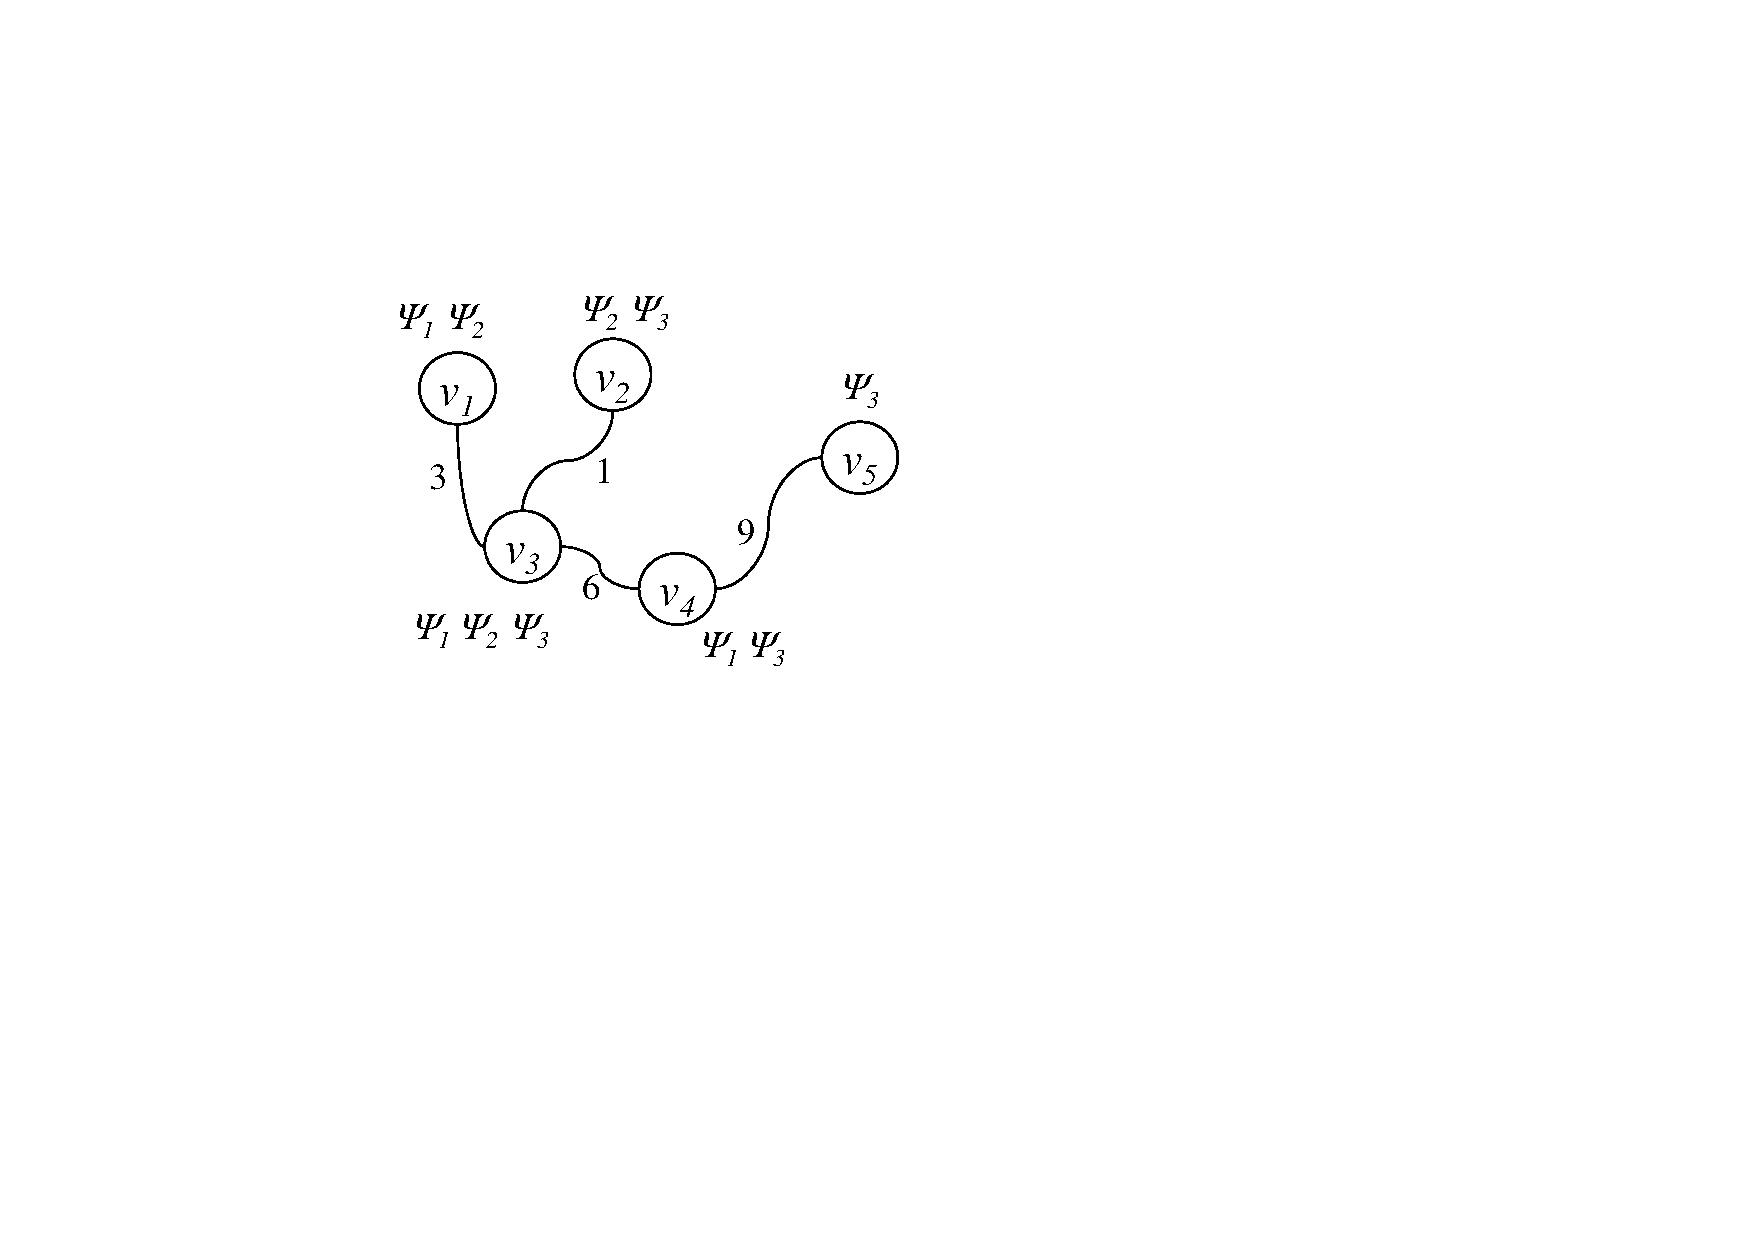
\includegraphics[width=0.45\columnwidth]{images/cachegraph}
    \end{tabular}
    \\
    %\hspace{1.5em}Inverted lists & 
    \hspace{1em}Graph representation &  \hspace{1.5em}Prefix compressed & Visualization
  \end{tabular}
\end{figure}
}}

\end{frame}
%
\subsection{Incremental update optimization}\label{sec:optIncUpd}

According the protocol when one (or more) location or vicinity enclosing
granule changes due to user movement, user's encrypted data must
be updated on the \ls by sending a $M_{el}$ message. Thus, in most
cases user's two consecutive $M_{el}$ messages would contain duplicated 
encrypted granules. 

The communication can be reduced by enabling so called \textit{incremental
updates}(\iuns). Here we introduce new type of message $M_{elUpd}$ that clients 
are allowed to send, instead of the $M_{el}$, when their locations change. 
It contains old items $u$, $l$, $g^*_l$ from $M_{el}$ and new items 
$\mathbf{g^*_{vDel}}$, $\mathbf{g^*_{vIns}}$, where $\mathbf{g^*_{vDel}}$, 
$\mathbf{g^*_{vIns}}$ define encrypted granules that must be deleted and inserted 
on the \ls in order to fully update some user $u$ encrypted data for level $l$. 
More precisely, if $m_1$ and $m_2$ are two consequent messages of type 
$M_{el}$ such that $m_1.u$=$m_2.u$ and $m_1.l = m_2.l$ then the
client may send a message $m_3$ of type $M_{elUpd}$ instead of $m_2$, where
$m_3.\mathbf{g^*_{vDel}}$ = $m_1.\mathbf{g^*_{v}}$
$\backslash$ $m_2.\mathbf{g^*_{v}}$ and $m_3.\mathbf{g^*_{vIns}}$ =
$m_2.\mathbf{g^*_{v}}$ $\backslash$ $m_1.\mathbf{g^*_{v}}$. 
Figure \ref{fig:ui_rf}a visualizes locations, vicinities, and 
vicinity-intersecting granules of user $u$ at two consequent 
time steps 0 and 1. Darkened sets of cells $\mathbf{g_{vDel}}$ and 
$\mathbf{g_{vIns}}$ visualize unencrypted representation of sets $g^*_{vDel}$ 
and $g^*_{vIns}$. Note, that introduction of $m_3$ helps reducing communication
only if $|m_3.\mathbf{g^*_{vDel}}|$ + $|m_3.\mathbf{g^*_{vIns}}|$ $<$
$|m_2.\mathbf{g^*_{v}}|$. 


Our presented client and server algorithms (See Alg. \ref{algCl}, \ref{algSrv})
can be easily modified to support incremental updates. In the current
implementation once a user goes from higher to lower levels (switches into
coarser granularity) granules of active level are being removed from stacks
on client and server ($GS$ and $GL$) without possibility to reuse them. The idea
is to preserve these granules on both client and server such that it would be
possible to update them utilizing $\mathbf{g_{vDel}}$, $\mathbf{g_{vIns}}$ or
$\mathbf{g^*_{vDel}}$, $\mathbf{g^*_{vIns}}$. 

The incremental updates impact on client communication is evaluated in 
Sec. \ref{sec:performStudy}.


\subsection{Grouping of Users}\label{subsec:grouping}

Currently all users in $\mathbf{M}$ share a single encryption function $\Psi$.
Security of $\Psi$ directly influence location privacy of all users in the
system. An adversary knowing $\Psi$ can easily decipher encrypted
granules of user current location and his vicinity. It is difficult to ensure
that the function $\Psi$ will stay secret in case of a high number of users
of the \vl service. Note that in case of leaked $\Psi$ users' minimum privacy 
requirements, specified by $L_{max}$, are still guaranteed, although it is 
desirable for users to obtain as much privacy as possible.

In order to limit affected users in case of leaked $\Psi$
\textit{grouping of users} can be enforced. Friend-grouping is
introduced in the long-paper version of the \ff \cite{ffinder}. The idea is
that all users in the system are grouped into possibly overlapping groups, so
that each user is put into one or more groups. Both friends and non-friends can
belong to the same group, but if two users are friends, they must be in at least
one common group. Each such group $G$ is assigned a distinct $\Psi_G$ function
and it is used by all members of $G$. Then if such $\Psi_G$ is leaked, only the
location privacy of the users in group $G$ are compromised.

Our presented algorithms of \vl can be easily modified to support friend
groups. The client and the server should treat each group individually such
that clients report their encrypted data for all groups that they are part of,
and the server independently analyzes encrypted data for every distinct group. 
In this paper, we do not consider how these groups are created. This can be done
automatically or manually by the users themselves.

%\input{articleFiles/rasterapproach.tex}
\section{Vulnerabilities \& Points of Attack}\label{sec:vulnerability}
We here address a few of the possible vulnerabilities
of the \vl approach. We assume correct behavior of both
the server and clients, and thus exclude attacks where an
attacker may want to modify either server or client to
e.g. trigger a ``spamming'' behavior.
The attackers goal will for each attack be to 
compromise the privacy of the largest possible number of
clients in the \vl system. 


\subsection{Compromised Client}\label{subsec:VulClient}
If an attacker gains control over a client
he will, for each group (see \ref{subsec:grouping})
the client is member of, have the $\Psi$ function 
used to calculate granules at the client.

If the client itself is compromised by an attacker, the $\Psi$ function
is not much help to him, since he cannot do much else than encode granules
sent to the server, but if one imagines that the attacker only temporarily
gains control, then he can use the $\Psi$ function to ``Clone'' the original
client. This problem is however easily made void by changing the $\Psi$ 
function regularly.

By using the \textit{battleship} method 
the attacker can guess the location of other users with same group 
membership as the compromised client\footnote{In the game of \textit{battleships} 
two opponents take turn to guess the location of the others battleships placed at 
secret locations in a grid.}.

One way an attacker may ``play battleship'' in order to find the location of
other users (with same group membership) would be to send a 
false vicinity covering the area he is interested in finding
other users, the attacker will then be notified by the server if any other 
user is within his false vicinity. The attacker then continues to cut the vicinity in half,
doing a binary search until he has found the granules of all users within the larger area
he initially sent his false vicinity for at the start\footnote{The amount of 
granules needed to be searched in the worst case is $\frac{c^{l+1}-1}{c-1}$ 
where $l$ is the number of levels needed to be traversed, and $c$ the number 
of granules each granule at level $l$ is divided into at $l+1$}.

By using groups this attack is already very limited, since each 
client is assumed to have far fewer friends then the overall amount
of users in the \vl system. Furthermore it is worth noticing that 
the attacker can never get an actual location of a user, since all he can get
a matching granule which corresponds to a spacial area and not a point.
There is also a build in limit on the amount of precision the attacker 
can achieve because each users $L_{max}$ is a limit on the precision that
any user will reveal. 
 
If we limit the attackers goal to only focus on a single friend, then 
using the binary search method described will enable the attacker to
track the single friend with the amount of vicinity splits he have to
do in worst case being: $\Theta(Log(\frac{B(cg)}{B(max)}))$ where $B(cg)$ is the
size of attackers current granule and $B(max)$ is the granule size at the maximum
precision attacker can get, either by setting his own $L_{max}$ or reaching the 
friends $L_{max}$.



\subsection{Compromised Server \& Client}\label{subsec:VulCliServ}
If the attacker has gained control over both the server and 
client, he has all info from \ref{subsec:VulClient} as well as 
all users encrypted center and vicinity granules, as well
as their group memberships (see \ref{subsec:grouping}).

The attacker can do the same as in \ref{subsec:VulClient}, 
only now the attacker can skip the \textit{battleship} step and decode
obfuscated location (center granules) of friends directly, making it
actually feasible to track all friends, this however is still
only valid for the groups that the compromised client is member of.

This attack has the same limitations as \ref{subsec:VulClient}, except
that since the attacker now skip the \textit{battleship} stage, it is 
feasible for the attacker to track many users (as long as they are in the
same group as the compromised client)
%
%\subsection{History}\label{subsec:VulHis} \ffh{not relevant, not risk}
%\textbf{info:} All users encrypted center and granules, 
%as well as their group memberships. The attacker collects data over time.
%
%\textbf{can do:} he can try to reason about how the center granule
%moves, by assuming it only moves a cell at a time,
%but this assumption does not hold so attacker can
%really reason about routes unless he has extra info
%about user (e.g. that user is from a specific region of a country,
%then he can maybe brute force possibilities in relation to road networks)


\subsection{Frequency}\label{subsec:VulFreq}
In this attack the server is compromised, and thus the
attacker knows all users encrypted center and granules, 
stored on the server, as well as their group memberships. 

The attacker can compare the frequency of users with same center and 
vicinity granules, the attacker can then see if many users
have the same granules, and reason about the actual location
(e.g. if attacker knows the national soccer team is playing, and he can
see many users suddenly all sharing granules).
The attacker can possibly collect the data over time and maybe make this attack
more efficient by looking for frequency in locations over time, e.g. if 
there is a central place most people must pass during the day (city center/a bridge etc.), 
the attacker can then use historical information to identify which granules 
correspond to this location.

There is a simple solution to thwart the effectiveness of this attack, and that is
to change the $\Psi$ function as some interval, making it impossible for the attacker
to compare granules from different intervals. If we furthermore assume that the server
would not be informed when $\Psi$ function is changed, then this attack becomes void.




\section{Experiments}\label{sec:experiments}
%
In this section, we evaluate the performance of our methods with our competitors on real datsets.
% We will conduct experiments
We have implemented two variants of our methods (SPC and SPC*).
%for extracting statistics of queries, benchmarking the cost of a shortest path call,
%and selecting promising paths from a query log $\mathcal{QL}$ into the cache.
They share the same techniques in Section~\ref{sec:BenefitDriven},
and only differ in their cache structures:
(i) SPC uses a path array cache (Section~\ref{sec:cacheLookup}), and (ii) SPC* uses the compressed graph cache (Sections~\ref{sec:cacheSubgraph},\ref{sec:cacheCompress}).
%
Our competitors are LRU (a dynamic caching method) and HQF (a static caching method).
They have been introduced in Section~\ref{sec:competitors}.
All the above methods are written in C++.
We conduct our experiments on an Intel i7 3.4GHz PC running Debian.

%  (ii) SPC$^+$ uses a graph cache (Section~\ref{sec:cacheSubgraph}),
%SPC, our method, with the 3 cache representation schemes - List cache, Graph cache, Compressed Graph cache - described in section

We will evaluate the above methods for a cache located at the proxy, and for a cache located at the server.
For the proxy scenario, the performance measure is the hit ratio.
For the server scenario, the performance measures are: (i) the total running time of the server,
and (ii) the total number of road network nodes visited.


%in both the proxy
%well both when considering the Proxy and Server scenario

%To compare how well we have done, we have implemented two baseline competitors, LRU and HQF. LRU is a dynamic caching method which evicts the Least recently used cache item if there is no space in the cache for new entries. HQF adds to the cache, the \spaths from the most frequent start-/end-points in the training data.





%Aalborg: total nodes in SPs from training set: 352032 in 1643 paths

%Beijing: total nodes in SPs from training set: 316400 in 6479 paths



%This is the most common usage of static caching in the web caching literature \cite{BaezaYates07}.


% In this section, we present the results of performance
% experiments, demonstrating the efficiency and realworld applicability of the proposed algorithms. We


\subsection{Experimental Setting}
%
We are unable to obtain real query log from online shortest path services (e.g., Google Map), due to their privacy policies.
Thus, we can only simulate a query log from a trajectory dataset.
For each trajectory, we extract its start location and its end location as the
source $v_s$ and destination $v_t$ of a shortest path query respectively.

We have used two real datasets and their details can be found in Table~\ref{tab:datasetsize}.
Each dataset consists of (i) a collection of trajectories (which can be used to simulate a query log), and 
(ii) a corresponding road network for the trajectories.

%Which historical query datasets do we have, and what is their size and origin.

%- Aalborg: Query workload from and around the Danish city of Aalborg

%- Beijing: Query workload from Beijing



Following the experimental methodology of static caching~\cite{Ozcan2011},
we divide the query log into two equal sets.
The {\em historical query log} set is used for defining query frequencies and
for filling the cache content.
The {\em query workload set} set can only used for testing the performance of our method.


%We do not give a default size for the query-datasets Maps, as we will execute all of our tests, described in section \ref{subsec:expProxy} and \ref{subsec:expServer}, for each dataset.


\begin{table}
\center
\begin{tabular}{|c|r|r|r|}\hline
Dataset & $\#$ Trajectories / Queries & $\#$ Nodes & $\#$ Edges \\\hline
Aalborg & 4.401  & 129.680 & 137.470 \\\hline
Beijing & 12.928 & 76.226 & 85.882 \\\hline
\end{tabular}
\caption{Description of real datasets}
\label{tab:datasetsize}
\end{table}
%% Aalborg = Aalborg
%% Beijing = Beijing


%GPS trajectories

%according to XXX l

%The size of training and test query datasets are given already. The size of each dataset, as well as the map they are captured on, is given in table \ref{tab:datasetsize}.



%% Aalborg = Aalborg
%% Beijing = Beijing


%We do not give a default size for the query-datasets Maps, as we will execute all of our tests, described in section \ref{subsec:expProxy} and \ref{subsec:expServer}, for each dataset.




All caching methods, SPC, SPC*, HQF, and LRU, share a number of common settings which, unless stated otherwise, will be set to their default values:
The number of levels in the kD-tree is 14 (i.e. 16,384 regions). We will use the list cache representation as the default cache representation, where each vertex use one byte. The default cache size is set to 625 kB.


The default cache size, as well as the maximum cache size in later experiments (Fig.~\ref{fig:cSizeVsHitRatio}, \ref{fig:cacheSizeVsHitRuntime}, \ref{fig:cacheSizeVsNodesvisited}), is choosen baring in mind the size of the Aalborg and Beijing query logs. 
Had we had access to large datasets of real query logs, from online shortest path serveice providers, we would use a large cache size like 1 GB.

% 
% 
% The size of our datasets is the limiting factor
% 



\label{fig:cacheSizeVsHitRuntime}

\label{fig:cacheSizeVsNodesvisited}


% - Which parameters are common for all tests
% - What are the ranges/values each parameter can take.
% - Which parameters are set to a default value unless otherwise stated (and what are the default values)
% - Which methods, and in which configuration, do we consider.



\subsection{Caching in the Proxy Scenario}\label{subsec:expProxy}
%
In the proxy scenario, the shortest path call API would issue a shortest path query to the server,
rather than performing computation by itself (see Section~\ref{sec:benchmark}).
Since the total cost is dominated by the communication round-trip time with server,
we use the cache hit ratio as the performance measure in this scenario.

For both datasets we vary the cache size and kD-tree levels to show the impact on the cache hit ratio. We have implemented a number of optimizations to the cache storage (See sec. \ref{sec:CacheStruct}) and show their impact on the cache hit ratio.


\stitle{Effect of the cache size}
%
In Figure~\ref{fig:cSizeVsHitRatio}, we measure the hit ratio of the methods
while varying the cache size from 1 kB to 5 MB.


\begin{figure}[htb]
\center
  \begin{tabular}{@{}c@{ }c@{}}
     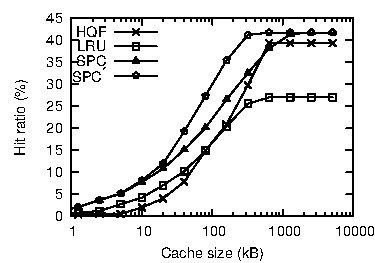
\includegraphics[width=0.5\columnwidth]{figures/cachesize_hitratio_aal.pdf}
     &
     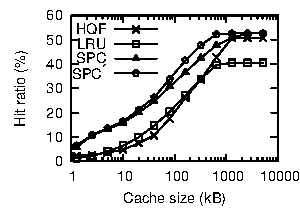
\includegraphics[width=0.5\columnwidth]{figures/cachesize_hitratio_bei.pdf}
      \\
     (a) Aalborg & (b)  Beijing
     \end{tabular}
\caption{Hit ratio vs. cache size }
\label{fig:cSizeVsHitRatio}
\end{figure}

% \begin{itemize}
% \item We can see SPC* performs much better than competitors
% \item LRU perform well on small cache sizes, but the cache hit ratio quickly level out and stop growing, thus LRU is not scalable.
% \item HQF performance is very consistent, with the hit ratio varying only slightly. The hit ratio does however stay at just over 1\% for Aalborg experiments and around 0.2\% for Beijing experiments. It is not usable
% \item We observe that SPC initially does not grow as fast as LRU, but the growth continues as we increase cache size, unlike for LRU.
% \item SPC* grows faster than LRU and gets better cache hit ratio at all cache sizes than LRU and SPC, except for the smallest cache size.
% \item The test on the Aalborg vs. Beijing sets show that SPC performs much better on the Aalborg set, where as LRU performs about 50\% worse. This can be explained by the fact that both methods rely on users behaving consistently over time, but where SPC relies on global consistency in user behavior, LRU need local consistency too. This makes SPC/SPC* more robust and we can expect them to always outperform LRU.
% \end{itemize}
{\color{red}
We can see that LRU consistently perform worse than SPC and SPC$^*$ for all cache sizes. The cache hit ratio stabilizes at about 26 and 40\% for Aalborg and Beijing respectively. Since LRU levels out at a much lower cache hit ratio than all of it's competitors it is not a suitable choice for \spath cacheing.


The performance of HQF is quite low at smaller cache sizes, 

The performance of HQF is very consistent, with the hit ratio varying only slightly. The hit ratio stays at just over 1\% for Aalborg experiments and around 0.2\% for Beijing experiments. The low hit ratio makes it not scalable and unusable for \spath caching.
}

SPC does not grow as fast as LRU for smaller cache sizes, but while the growth of LRU quickly stabilizes then SPC continues to grow and outperforms both LRU and HQF.
SPC* outperforms both LRU and SPC by a large margin, only shortly having a lower cache hit ratio at smaller cache sizes. The test on Aalborg vs. Beijing  show that SPC performs much better on the Aalborg set, where as LRU performs about 50\% worse. This can be explained by the fact that both methods rely on users behaving consistently over time, but where SPC relies on global consistency in user behavior, LRU need local consistency too. This makes SPC/SPC* more robust and we expect them to always outperform LRU.



\stitle{Effect of the kD-tree level}
%
In Figure~\ref{fig:levelVsHitRatio}, we vary the kD-tree level from 8 to 18 levels and show that using a kD-tree of about 14 levels can significantly increase the cache hit ratio of both the Aalborg and Beijing dataset. SPC* performs better than SPC.


\begin{figure}[htb]
\center
  \begin{tabular}{@{}c@{ }c@{}}
     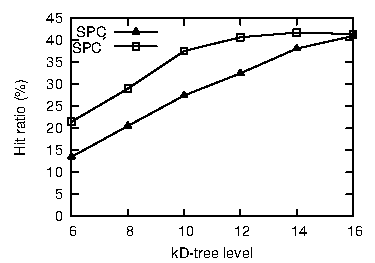
\includegraphics[width=0.5\columnwidth]{figures/split_hitratio_aal.pdf}
     &
     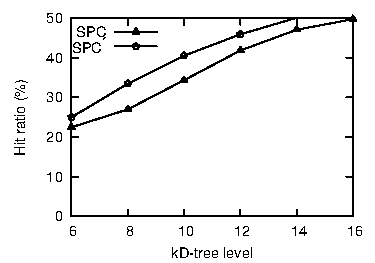
\includegraphics[width=0.5\columnwidth]{figures/split_hitratio_bei.pdf}
      \\
     (a) Aalborg & (b)  Beijing
     \end{tabular}
\caption{Hit ratio vs. Levels}
\label{fig:levelVsHitRatio}
\end{figure}

On both dataset SPC* outperforms SPC by a large margin. On the city X dataset SPC* achieves more than a 50\% increase in hit ratio, and when compared to SPC, it achieves a relative performance gain of 500-900\% at low levels up to the peak performance at level 14.
On the Y dataset SPC* gets a lower hit ratio, but it still achieves more than 50\% cache hit ratio. The results are still very impressive, with SPC* performing 200-400\% better than SPC at all levels.

% \noindent
% \begin{tabular}{|l |p{0.58\columnwidth} |l |}
% \hline
% \textbf{Parameter} & \textbf{Meaning / used for} & \textbf{Standard value} \\\hline
% Mapfile & The map which the test is performed on & \\\hline
% NumQueries & Number of \spath queries in test & \\\hline
% QuerySet & which dataset is used to provide queries & \\\hline
% TrainSet & For generating region statistics, which dataset is used & \\\hline
% CacheSize & Size of cache in bits & \\\hline
% cacheType & Type of cache representation (list/graph) & \\\hline
% kD-tree & Hight of the kD-tree & \\\hline
% avgLenght & Average length of a shortest path & \\\hline
% \end{tabular}

% Write experiments to examine performance of goal 1 \& 2
% Test ideas (several ideas may be combined, like item 1 can be done on all datasets from item 2):\\
% \begin{itemize}
% \item increase kd-tree hight from 0-18
% \item different maps [Oldenburg, Aalborg, Beijing]
% \item compare cache type performance
% \item compare with baseline methods. [LRU dynamic, Dynamic(maxLevel)]
% \item vary the cache size [10.000-2560000]
% \item vary number of queries. [only for synthetic data]
% \end{itemize}

\subsection{Caching in the Server Scenario}\label{subsec:expServer}
%
In the server scenario, the shortest path API has to invoke a shortest path algorithm.
Thus, the running time is the most important performance measure. We also measure the number of nodes visited in a shortest path algorithm, which serves an indicator of the running time.
%On a server our aim is slightly different than on the Proxy, as we also have to consider that there may be some paths that are so small that it may be cheaper to simply re-calculate the result, instead of caching it.
%For the server scenario we will test the cache hit ratio, running time, and Nodes visited.
%For all three experiments
%We will vary kD-tree levels and cache size in the following experiments.
As a case study, we use the Dijkstra's algorithm as the shortest path algorithm.

In the following experiments, the running time (and nodes visited) refer to the total running time (and nodes visited) for processing the entire query workload. The running time is measured in the unit of seconds.





\stitle{Estimation of shortest path running cost}
%
First, we test the estimation error of our cost estimation technique proposed in Section~\ref{sec:benchmark}.
We measure the error percentage in terms of the relative error between the actual cost and the estimated cost.
Table~\ref{tbl:estcost} shows the estimation error of our technique
as a function of: (a) the number of landmark $|U|$, and (b) the size of the samples $S$.
The default values are: $|U|=20$ and $S=100$.
The majority of errors are below 30\% and thus our estimation technique is reasonably accurate.


%% Aalborg: average cost = 136347/2 = 68173
%%  Beijing: average cost = 79603/2 = 39801
%  average because random node chosen



\begin{table}
\center
\begin{tabular}{cc}
    \begin{tabular}{|c|c|c|}
    \hline
    $|U|$ & Aalborg & Beijing \\ \hline \hline
     5 & 35.5 & 33.3 \\ \hline
     10 & 25.4 & 28.2 \\ \hline
     20 & 22.2 & 23.9 \\ \hline
     40 & 19.4 & 23.0  \\ \hline
     80 & 19.9 & 21.9 \\ \hline
    \end{tabular}
    &
    \begin{tabular}{|c|c|c|}
    \hline
    $S$ & Aalborg & Beijing \\ \hline \hline
     25 & 23.4 & 28.8 \\ \hline
     50 & 20.7 & 28.4 \\ \hline
     100 & 22.2 & 23.9 \\ \hline
     200 & 20.4 & 22.7 \\ \hline
     400 & 21.1 & 21.3 \\ \hline
    \end{tabular}
    \\
    (a) varying number of landmark $|U|$ & (b) varying sample size $S$
\end{tabular}
    \caption{Average error percentage of cost estimation}
    \label{tbl:estcost}
\end{table}








%
\stitle{Effect of the kD-tree level}
%
In Figure~\ref{fig:levelVsHitRatio}, we again vary the kD-tree level from 8 to 18 levels. All three experiments shows a consistent advantage of using SPC* over SPC. SPC* still has an even higher advantage than in the proxy scenario, performing around 950\% better than SPC at its best. SPC, however, has a very low hit ratio in the server scenario, on both the city X and Y datasets. In figure \ref{fig:levelVsruntime}a and b we can see that SPC* is very fast at answering the query workload. SPC has a quite stable time in both figure\ref{fig:levelVsruntime}a and b, while the time for SPC* to answer the query workload actually decreases with more regions. In figure \ref{fig:levelVsNodesvisited} we can see that SPC* visits far fewer nodes than SPC, during shortest path calculations. This is expected since SPC* can answer many more queries from its cache.




\begin{figure}[htb]
\center
  \begin{tabular}{@{}c@{ }c@{}}
     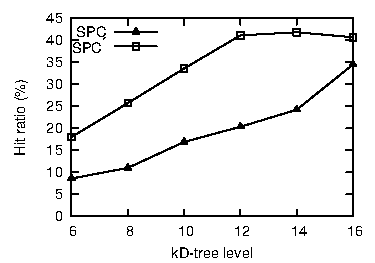
\includegraphics[width=0.5\columnwidth]{figures/split_hitratio_aal_server.pdf}
     &
     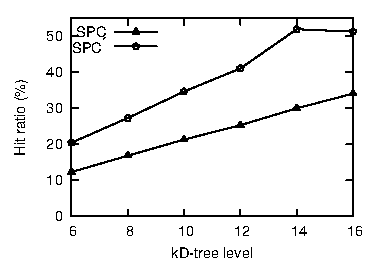
\includegraphics[width=0.5\columnwidth]{figures/split_hitratio_bei_server.pdf}
      \\
     (a) Aalborg & (b)  Beijing
     \end{tabular}
\caption{Hit ratio vs. Levels}
\label{fig:levelVsHitRatio}
\end{figure}

\begin{figure}[htb]
\center
  \begin{tabular}{@{}c@{ }c@{}}
     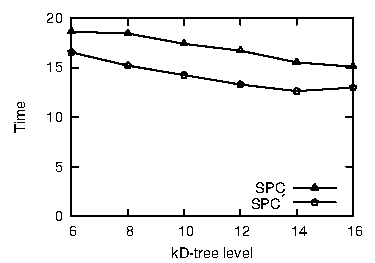
\includegraphics[width=0.5\columnwidth]{figures/split_runtime_aal_server.pdf}
     &
     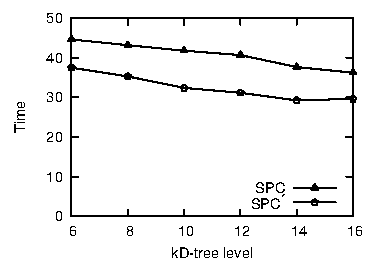
\includegraphics[width=0.5\columnwidth]{figures/split_runtime_bei_server.pdf}
      \\
     (a) Aalborg & (b)  Beijing
     \end{tabular}
\caption{Runtime vs. Levels}
\label{fig:levelVsruntime}
\end{figure}

\begin{figure}[htb]
\center
  \begin{tabular}{@{}c@{ }c@{}}
     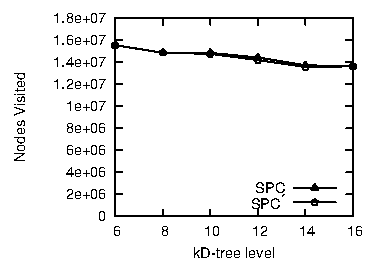
\includegraphics[width=0.5\columnwidth]{figures/split_nodes_aal_server.pdf}
     &
     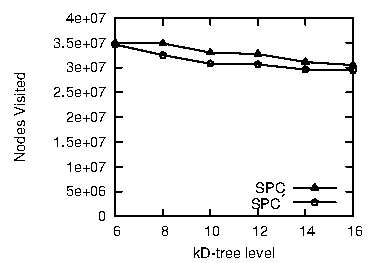
\includegraphics[width=0.5\columnwidth]{figures/split_nodes_bei_server.pdf}
      \\
     (a) Aalborg & (b)  Beijing
     \end{tabular}
\caption{Nodes Visited vs. Levels}
\label{fig:levelVsNodesvisited}
\end{figure}






\stitle{Effect of the cache size}
%
In the following experiments, we vary the cache size and observe the effect on the running time and nodes visited during shortest path calculations.






\begin{figure}[htb]
\center
  \begin{tabular}{@{}c@{ }c@{}}
     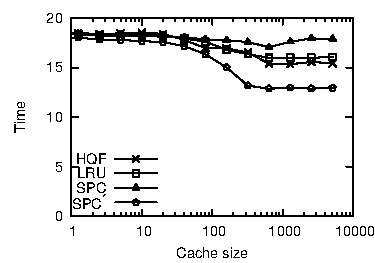
\includegraphics[width=0.5\columnwidth]{figures/cachesize_runtime_aal.pdf}
     &
     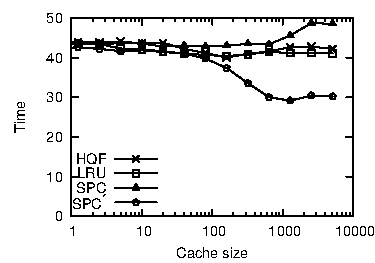
\includegraphics[width=0.5\columnwidth]{figures/cachesize_runtime_bei.pdf}
      \\
     (a) Aalborg & (b)  Beijing
     \end{tabular}
\caption{Runtime vs. Cache Size}
\label{fig:cacheSizeVsHitRuntime}
\end{figure}

In Figure \ref{fig:cacheSizeVsHitRuntime} and \ref{fig:cacheSizeVsNodesvisited}, for both the city X and Y dataset,  we can see that the graph looks similar to Figure \ref{fig:cSizeVsHitRatio}, but in the upside-down manner. This is to be expected, since a higher cache hit ratio gives fewer \spath calculations, and a lower runnig time when answering queries.

\begin{figure}[htb]
\center
  \begin{tabular}{@{}c@{ }c@{}}
     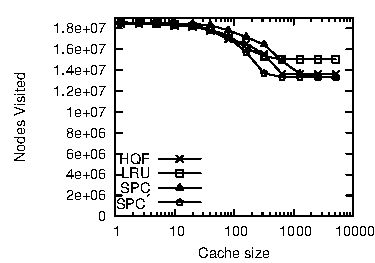
\includegraphics[width=0.5\columnwidth]{figures/cachesize_nodes_aal.pdf}
     &
     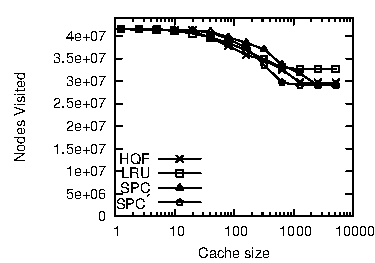
\includegraphics[width=0.5\columnwidth]{figures/cachesize_nodes_bei.pdf}
      \\
     (a) Aalborg & (b)  Beijing
     \end{tabular}
\caption{Nodes Visited vs. Cache Size}
\label{fig:cacheSizeVsNodesvisited}
\end{figure}

%\section{Future work} \label{sec:future}
Lorem ipsum dolor sit amet, consectetur adipiscing elit. Pellentesque elementum elementum turpis. Pellentesque diam elit, scelerisque eget, mollis vel, aliquet feugiat, dolor. Nunc dignissim tristique risus. Maecenas molestie tellus sit amet neque. Etiam porttitor posuere lacus. Etiam mi diam, dapibus hendrerit, condimentum in, malesuada eget, libero. Aliquam enim. Nam dolor dolor, fermentum et, faucibus sodales, iaculis sed, justo. Integer sagittis placerat justo. Cum sociis natoque penatibus et magnis dis parturient montes, nascetur ridiculus mus. Donec ullamcorper metus at turpis. Proin vel risus. Nam libero lectus, gravida vel, aliquet a, vestibulum a, lorem. Mauris eget quam non enim placerat consequat. Nam dolor lacus, lacinia et, posuere vitae, sollicitudin vel, eros.
\section{Conclusion and Future Work}\label{sec:future}



summation of each goal from the problem setting for each goal argue we solved it well (recap key results and partial conclusions from applicable sections).






% In this paper we develop a novel Privacy Profile which enable users to easily specify their privacy requirements both spatially and temporally for trajectories.
% 
% To show the Privacy Profile usefull we develop framework with a high level of user privacy and providing a platform for service providers and traffic analysts to have high quality data to perform analysis and services on.
% 
% We have argued that the Privacy Profile provide: 
% {\it Usability} The user can specify his privacy requirements both spatially and temporally, and at more than one level. Is {\it Practical} The user does not need to interact with the client once a Privacy Profile is set up. The data input format is the same as the data output format making the anonymized data usable by existing approaches working on trajectory datasets allowing the user to choose from more existing services. It is {\it Flexible} Users can specify sensitivity at several levels and they can make several profiles which are active at different times or in contexts.
% 
% We have additionally introduced the system parameter $\mathbf{D}$ which guaranties a minimum level of data integrity, ensuring that analysis of the anonymized dataset can still be possible.
% 
% In the future it would be interresting to test the approach on real world trajectory dataset to measure performance and examine which values of $D$ might be appropriate to ensure a level of data quality usable by existing classification approaches for trajectories.

%-------------------------------------------------------------------------

\bibliographystyle{splncs}

\bibliography{bibliography}

\end{document}